\documentclass{beamer}
%\documentclass[notes]{beamer}
%\documentclass[notes=only]{beamer}
\usepackage[utf8]{inputenc}
\usepackage{tikz}
\usetikzlibrary{arrows.meta}
\tikzset{>={Latex[width=2mm,length=2mm]},
  base/.style = {
    rectangle, rounded corners, draw=black,
    minimum height=1cm, text centered, font=\sffamily
  },
  process/.style = {
    base, minimum width=2.5cm, fill=orange!15,
    font=\ttfamily
  },
}

\graphicspath{{./img/},{../2021_05/img/},{../2020_03/img/}}
\DeclareGraphicsExtensions{.png,.jpg,.pdf}

\usepackage{hyperref}
\hypersetup{colorlinks,urlcolor=blue!50!black,linkcolor=red}

\usepackage{fontawesome}
\usepackage{listings}

\title{\small Máster en Sistemas Electrónicos Avanzados (MSEA)\\\Large Co-simulación y verificación funcional con\\VHDL, C/C++ y Python/m\\{\small $\{$main$\}$}}
\author{Unai Martinez Corral\\\href{mailto:unai.martinezcorral@ehu.eus}{\faEnvelope~unai.martinezcorral@ehu.eus}\\\href{https://orcid.org/0000-0003-1752-9181}{\faGlobe~ORCID} ~\href{https://github.com/umarcor}{\faGithub~umarcor} ~\href{https://gitlab.com/umarcor}{\faGitlab~umarcor}}
\institute{Escuela de Ingeniería de Bilbao\\Universidad del País Vasco/Euskal Herriko Unibertsitatea (UPV/EHU)}
\date{2022/05}

\begin{document}

\frame{\titlepage}

\begin{frame}
\frametitle{Academic background}
\small
\vfill
\begin{itemize}
\item
  2013.
  \emph{Ingeniería Técnica Industrial, Esp. Electrónica Industrial}.
  Escuela de Ingeniería Técnica Industrial (EUITI) in Bilbao.
  University of the Basque Country (UPV/EHU).

\vfill

\item
  2015.
  \emph{Máster en Sistemas Electrónicos Avanzados (SIEAV)} \href{https://www.ehu.eus/es/web/master/master-sistemas-electronicos-avanzados}{\faGlobe}.
  Doctoral School, Faculty of Engineering in Bilbao.
  University of the Basque Country (UPV/EHU).

\vfill

\item
  Since 2015.
  \emph{Doctoral Programme in Engineering Physics} \href{https://www.ehu.eus/en/web/doktoregoak/doctorate-engineering-physics}{\faGlobe},
  advised by Prof. Koldo Basterretxea.
  Digital Electronics Design Group (GDED).
  University of the Basque Country (UPV/EHU).

\vfill

\item
  2018.
  \emph{Visiting Researcher},
  advised by Prof. Mikel Luján.
  Advanced Processor Technologies Research Group (APT) \href{http://apt.cs.manchester.ac.uk/}{\faGlobe}.
  University of Manchester.
\end{itemize}
\vfill
\end{frame}

\begin{frame}
\frametitle{Open Source background}
\small
\vfill
\begin{itemize}

\item Organisations in GitHub:

  \begin{tabular}[h]{ccc}
  \emph{Admin/owner} & \emph{Co-maintainer} & \emph{Member}
  \\

  HDL \href{http://github.com/hdl}{\faGithub}
  &
  GHDL \href{http://github.com/ghdl}{\faGithub}
  &
  SymbiFlow \href{https://github.com/SymbiFlow}{\faGithub}
  \\

  VHDL \href{http://github.com/vhdl}{\faGithub}
  &
  VUnit \href{http://github.com/VUnit}{\faGithub}
  &
  verilator \href{https://github.com/verilator}{\faGithub}
  \\

  DBHI \href{http://github.com/dbhi}{\faGithub}
  &
  &
  ITSAS \href{https://github.com/itsas-taldea}{\faGithub}
  \\
  \end{tabular}

\vfill

\item \emph{Secretary} of the VHDL Analysis and Standardisation Group (VASG), aka IEEE-P1076 \href{https://gitlab.com/IEEE-P1076}{\faGitlab}.

\vfill

\item Contributor to
  MSYS2 \href{https://github.com/msys2}{\faGithub},
  GTKWave \href{https://github.com/gtkwave/gtkwave}{\faGithub},
  Verilog-to-Routing \href{https://github.com/verilog-to-routing}{\faGithub},
  Microwatt \href{https://github.com/antonblanchard/microwatt}{\faGithub},
  I'm TOMU/FOMU \href{https://github.com/im-tomu}{\faGithub},
  Cobra \href{https://github.com/spf13/cobra}{\faGithub},
  etc.

\vfill

\item Awarded the Google Open Source Peer Bonus in Q1 2021 \href{https://opensource.googleblog.com/2021/04/announcing-first-group-of-google-open-source-peer-bonus-winners.html}{\faGlobe}.

\end{itemize}
\vfill
\end{frame}

\begin{frame}
\frametitle{19XX - 20XX}
\centering
\Huge
Software {\color{red}\bfseries/=} Hardware
\end{frame}

\note[itemize]{
\item El desarrollo software y el desarrollo hardware son diferentes.
\item No es lo mismo una aplicación JS/TS en Electron o un acelerador hardware en RTL.
\item Aplicaciones, sistema, drivers, arquitectura, microarquitectura, ...
\item Utilizamos diferentes lenguages, editores y herramientas en general.
\item La diferencia principal entre el "pensamiento hardware" y el "pensamiento software" radica en el modelo Von Neunman.
}

\begin{frame}
\frametitle{201X - $\infty$}
\centering
\Huge
Software {\color{green}\bfseries?=} Hardware
\end{frame}

\note[itemize]{
\item Bueno... quizá debieríamos decir "eran diferences" y "utilizábamos herramientas diferentes".
\item  Hay muchas más desarrolladoras de software que de hardware, además de programadores y makers.
\item  Tras la acumulación de datos en los 2000 y las limitaciones en la escalabilidad del modelo von neuman,
    las FPGAs han visto un auge significativo esta última decada.
\item  La atención de la comunidad de desarrollo de software ha traido de forma natural el interés de las comunidades open
    source y de software libre.
\item  Varios agentes han roto la baraja:
\begin{itemize}
  \item Las FPGAs son reprogramables, por lo que no hay razón para considerar el desarrollo de firmware/gateware diferente
    del software.
  \item Si el coste de fabricar un ASIC se reduce a cero, tampoco hay razón para considerar el desarrollo
    significativamente diferente.
\end{itemize}
}

\begin{frame}
\frametitle{EDA tooling ecosystem(s)}
\begin{center}
\includegraphics[width=.9\linewidth]{synthesis}

\vfill

hdl/awesome\#98 \href{https://github.com/hdl/awesome/issues/98}{{\faGithub}}
\end{center}

\vfill

{\tiny
Note:
Synthesis flows targeting FPGA bitstreams are shown only.
Simulation/verification and ASIC targets are not included in this diagram.

See also:
Rodrigo A. Melo.
\emph{Free and Open Source Software for FPGA development}.
February 2021.
\href{http://indico.ictp.it/event/9443/session/258/contribution/587/material/slides/}{\faSlideshare}
\href{http://indico.ictp.it/event/9443/session/258/contribution/587/material/video/}{\faVideoCamera}
}

\vfill

\end{frame}

\note[itemize]{
\item  En la última década han surgido y madurado toda una serie de proyectos para traer prácticas y herramientas utilizadas
   en el desarrollo de software y aplicarlas al desarrollo de hardware.
\item  Por razones geopolíticas y económicas, la mayoría de las mismas son open source (no necesariamente software libre).
\item  Con cierto delay (casi una década), las empresas relevantes del sector están uniéndose al "movimiento".

\item En estas sesiones vamos a hacer un repaso de las herramientas open source y libres más relevantes para el desarrollo y
   verificación de proyectos escritos en VHDL $>=$2008.
\item Vamos a centrarnos en la simulación, aunque haremos mención a la síntesis también.
}

\begin{frame}
\frametitle{Languages}
\vfill
\small
\begin{minipage}[t]{.49\linewidth}
\begin{itemize}
\item Dynamic/static
\item Interpreted/compiled
\item Strong/loose typing
\item Runtime
\item Memory management (GC)
\item Concurrency/parallelism
\end{itemize}
\end{minipage}
\begin{minipage}[t]{.5\linewidth}
\begin{itemize}
\item Assembly/ASM
\item Ada, C/C++, Java, C\#
\item go(lang), Rust
\item Python, m, Julia, Perl, Ruby
\item JavaScript, TypeScript
\item shell/bash, powershell, cmd
\item LaTeX/Tikz
\item MarkDown, reStructuredText
\item HTML, CSS/SASS
\item \ldots
\end{itemize}
\end{minipage}
\vfill
\centering
\href{https://en.wikipedia.org/wiki/Comparison_of_programming_languages}{\faWikipediaW~Comparison of programming languages}
\end{frame}

\note[itemize]{
\item Hay decenas, sino centenas, de lenguajes de programación, scripting y descripción.
\item Desde un punto de vista teórico, pueden organizarse en función de la sintaxis, los tipos, gestión de memoria, etc.
\item Algunos lenguajes son más adecuados para ciertas tareas o para capturar el conocimiento de algún area de estudio.
\item En ingeniería, es habitual tener que utilizar media docena de lenguajes, con más o menos frecuencia.
\item Sin embargo, todos los lenguajes se ejecutan sobre la misma máquina (arquitectura).
\item Todos los "programas" podemos escribirlos e interpretarlos en nuestros ordenadores, independientemente del uso final.
\item En cierta manera, todos son formas diferentes de representar lo mismo, ¿o no?
}

\begin{frame}
\frametitle{Languages: compilation and execution}
\centering
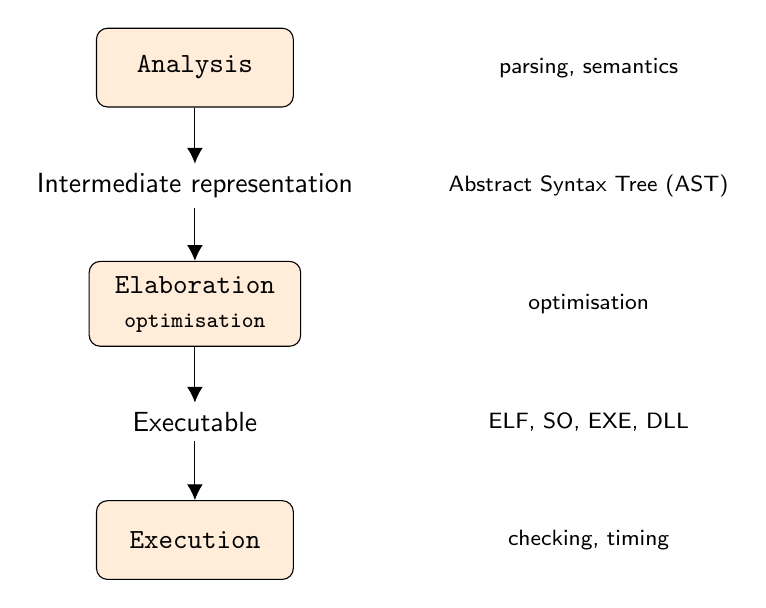
\begin{tikzpicture}[node distance=1.5cm, every node/.style={fill=white, font=\sffamily}]
  \node (ana) [process] {Analysis};
  \node (ana_i) [right of=ana, node distance=5cm] {\footnotesize parsing, semantics};
  \node (ast) [below of=ana] {Intermediate representation};
  \node (ast_i) [right of=ast, node distance=5cm] {\footnotesize Abstract Syntax Tree (AST)};
  \node (ela) [process, below of=ast] {\begin{tabular}{c}Elaboration\\\footnotesize optimisation\end{tabular}};
  \node (ela_i) [right of=ela, node distance=5cm] {\footnotesize optimisation};
  \node (bin) [below of=ela] {Executable};
  \node (bin_i) [right of=bin, node distance=5cm] {\footnotesize ELF, SO, EXE, DLL};
  \node (run) [process, below of=bin] {Execution};
  \node (run_i) [right of=run, node distance=5cm] {\footnotesize checking, timing};
  \draw[->] (ana) -- (ast);
  \draw[->] (ast) -- (ela);
  \draw[->] (ela) -- (bin);
  \draw[->] (bin) -- (run);
\end{tikzpicture}
\end{frame}

\note[itemize]{
\item Independientemente del lenguaje, todos los intérpretes o compiladores tienen una arquitectura parecida.
\item Análisis, elaboración y ejecución.
\item Los formatos concretos varían en función del lenguaje, sistema operativo, arquitectura.
}

\begin{frame}
\frametitle{Languages: unified compilation tools}
\vfill
\begin{itemize}
\item GNU Compiler Collection (GCC) \href{https://gcc.gnu.org/}{\faGlobe}
\item Low-level virtual machine (LLVM) \href{https://llvm.org/}{\faGlobe}; {\footnotesize despite its name, LLVM has little to do with traditional virtual machines.}
\end{itemize}

\vfill

\begin{itemize}
\item Java virtual machine (JVM) \href{https://en.wikipedia.org/wiki/Java_virtual_machine}{\faWikipediaW}
\item Dynamic Binary Modification/Translation (QEMU) \href{https://www.qemu.org/}{\faGlobe}
\item WebAssembly \href{https://webassembly.org/}{\faGlobe} \href{https://en.wikipedia.org/wiki/WebAssembly}{\faWikipediaW}
\end{itemize}
\vfill
\end{frame}

\note[itemize]{
\item Precisamente porque todos los intérpretes/compiladores tienen una arquitectura similar, existen proyectos para
   unificar y reutilizar los aspectos comunes.
\item GCC y LLVM son los compiladores de referencia, ambos software libre, que están soportados en decenas de arquitecturas
   y son utilizados por prácticamente cualquier proyecto (libre o incluso no-libre).
\item Asimismo, hay otros proyectos basados en la conversión de ciertas representaciones o instrucciones entre diferentes
   plataformas.

\item En general, proyectos compilados por diferentes herramientas pueden comunicarse entre sí utilizando interfaces
   específicas, y existen adaptadores entre dichas interfaces para diferentes plataformas.

\item ¿Cómo se incluyen los lenguajes de descripción de hardware en este esquema?
}

\begin{frame}
\frametitle{IEEE Hardware Description Languages}
\vfill
\begin{itemize}
\item 1076: \textbf{VHDL} (1987, 1993, 2000, 2002, 2008, 2019)
\item 1076.1: \textbf{VHDL-AMS} (1999, 2007, 2017)
\item 1364: \textbf{Verilog} (1995, 2001 2005)
\item 1800: \textbf{SystemVerilog} (2005, 2009, 2012, 2017)
\item 1850: Property Specification Language (\textbf{PSL}) (2005, 2010)
\item 1666: \textbf{SystemC} (2005, 2011, 2016)
\end{itemize}
\vfill
\centering
\Large\href{https://standards.ieee.org}{\faGlobe~standards.ieee.org}
\end{frame}

\note[itemize]{
\item Hay principalmente tres familias de lenguajes de descripción utilizados tradicionalmente en la industria:
   VHDL, (System) Verilog y SystemC.
\item Tanto VHDL como Verilog tienen extensiones para descripción de circuitos analógicos y para especificación de assertions.
}

\begin{frame}
\frametitle{HDL generators}
\begin{itemize}
\item High-Level Synthesis (HLS)
\href{https://en.wikipedia.org/wiki/High-level_synthesis}{\faWikipediaW}

\item Bluespec SystemVerilog (BSV) \href{https://bluespec.com/}{\faGlobe}
\href{https://github.com/bluespec}{\faGithub} \href{https://github.com/B-Lang-org/bsc}{\faGit}

\item Scala:
Chisel
\href{https://www.chisel-lang.org/}{\faGlobe} \href{https://github.com/freechipsproject/chisel3}{\faGithub},
SpinalHDL
\href{https://github.com/SpinalHDL}{\faGithub} \href{https://spinalhdl.github.io/SpinalDoc-RTD/}{\faBook}

\item Python:
MyHDL
\href{http://www.myhdl.org/}{\faGlobe} \href{https://github.com/myhdl/myhdl}{\faGithub},
Migen
\href{https://m-labs.hk/gateware/migen/}{\faGlobe}
\href{https://github.com/m-labs?type=source}{\faGithub},
nmigen
\href{https://nmigen.info/nmigen}{\faGlobe}
\href{https://github.com/nmigen/nmigen}{\faGithub},
Litex
\href{https://github.com/enjoy-digital/litex}{\faGithub}

\item Haskell:
Clash
\href{https://clash-lang.org/}{\faGlobe}
\href{https://github.com/clash-lang}{\faGithub}

\item Java:
Synthesijer
\href{https://github.com/synthesijer/synthesijer}{\faGithub}
\href{https://synthesijer.github.io/web/}{\faBook}

\item
Silice
\href{https://github.com/sylefeb/Silice}{\faGithub}

\item \ldots
\end{itemize}

\vfill

\begin{itemize}
\item Flexible Intermediate Representation for RTL (FIRRTL)
\href{https://github.com/freechipsproject/firrtl}{\faGithub}
\href{https://freechipsproject.github.io/firrtl/}{\faBook}
\end{itemize}
\end{frame}

\note[itemize]{
\item Sin embargo, especialmente esta última década, han surgido al menos una docena de lenguajes alternativos.
\item La mayoría son Domain Specific Languages (DSL) basados en un lenguaje de software existente.
\item Permiten expresar la funcionalidad y/o la estructura de los modelos y cosimularlos (verificarlos) junto con otras
   librerías escritas en el mismo lenguaje.
\item Adicionalmente, permiten exportar el diseño a Verilog y/o VHDL.
\item Es decir, se evita la cosimulación entre lenguajes diferentes, y por tanto, no se dispone de la certeza de la
   equivalencia del diseño con respecto a lo modelado.
\item Algunos, como SpinalHDL (o HDL Coder) sí permiten la cosimulación del HDL generado, para validar su corrección.
\item Para ello, es necesaria una herramienta de simulación HDL.
}

\begin{frame}
\frametitle{HDL simulation}
\vfill
\begin{itemize}
\item Mentor Graphics/Siemens, Intel-Altera: ModelSim/QuestaSim
\item Aldec: Active-HDL/Riviera-PRO
\item Xilinx: ISE ISIM, Vivado XSIM
\item Cadence: Incisive, Xcelium
\item Synopsys: VCS
\end{itemize}
\vfill
\centering
\href{https://en.wikipedia.org/wiki/List_of_HDL_simulators}{\faWikipediaW~List of HDL simulators}
\end{frame}

\note[itemize]{
\item Los simuladores HDL comerciales tradicionales permiten simular VHDL y/o System Verilog y/o SystemC.
\item La mayoría soportan una o varias interfaces de cosimulación, estandarizadas o no.
\item Sin embargo, el soporte del lenguaje VHDL es deficiente por razones económicas y políticas.
\item Al mismo tiempo, algunas características no están disponibles en las versiones gratuitas o en las licencias más
   asequibles.
\item Por lo tanto, existe un paywall nada despreciable para poder utilizarlos.
\item Asimismo, las licencias impiden discutir públicamente qué características están soportadas y cuáles no, lo cual
   dificulta el aprendizaje.
}

\begin{frame}
\frametitle{Circuit simulation: open source}
\begin{minipage}[t]{.58\linewidth}
HDL simulation:
\begin{itemize}
\item GHDL
\href{https://github.com/ghdl/ghdl}{\faGithub}
\href{https://ghdl.github.io/ghdl}{\faBook}

\item nvc
\href{https://github.com/nickg/nvc}{\faGithub}

\item Verilator
\href{https://www.veripool.org/wiki/verilator}{\faGlobe}
\href{https://github.com/verilator/verilator}{\faGithub}

\item Icarus Verilog (iverilog)
\href{http://iverilog.icarus.com/}{\faGlobe}
\href{https://github.com/steveicarus/iverilog}{\faGithub}
\end{itemize}
\end{minipage}
\begin{minipage}[t]{.405\linewidth}
Analog simulation:
\begin{itemize}
\item Xyce \href{https://xyce.sandia.gov/}{\faGlobe} \href{https://github.com/Xyce/Xyce}{\faGithub}
\item SPICE \href{https://en.wikipedia.org/wiki/SPICE}{\faWikipediaW}
\item Ngspice \href{http://ngspice.sourceforge.net/}{\faGlobe}
\item Gnucap \href{http://gnucap.org}{\faGlobe}
\end{itemize}
\end{minipage}

\vfill
Waveform visualisation:
\begin{itemize}

\item GtkWave (LXT, LXT2, VZT, FST, GHW, VCD/EVCD)
\href{http://gtkwave.sourceforge.net/}{\faGlobe}
\href{https://github.com/gtkwave/gtkwave}{\faGithub}

\item dwfv (VCD)
\href{https://github.com/psurply/dwfv}{\faGithub}
\end{itemize}

\end{frame}

\note[itemize]{
\item Existen herramientas open source para simulación de circuitos digitales y analógicos que ofrecen rendimiento y
   características comparables a las soluciones comerciales.
\item Nos permiten no sólo usarlas, sino entender qué se hace con el código HDL para obtener un modelo ejecutable (una
   simulación) o una netlist sintetizada.
}

\begin{frame}
\frametitle{HDL simulation: GHDL}
\small Free and open-source  analyser, compiler, simulator and experimental synthesiser for VHDL. GHDL is not an interpreter: it allows to generate machine code from design sources.

\vspace{1em}
\includegraphics[width=\linewidth]{ghdl-internals.pdf}
\vspace{.5em}

\tiny
\begin{itemize}
  \item Full support for the 1987, 1993, 2002 versions of VHDL, and partial for 2008. Partial support of PSL.
  \item Three backends: LLVM, GCC or, x86\_64/i386 only, a built-in one (mcode).
  \item GNU/Linux, Windows and macOS; on x86, x86\_64, armv6/armv7/aarch32 and aarch64.
  \item Can write waveforms (GHW, VCD or FST).
  \item Synthesis: plain VHDL or yosys (through ghdlsynth).
\end{itemize}
\end{frame}

\note[itemize]{
\item GHDL is a free and open source fully featured toolbox for VHDL.
\item It provides the most complete open source parsing/analysis of the language (better than several vendor tools).
\item It allows simulation, co-simulation and synthesis, apart from providing a Python interface and an LSP built on it.
\item Multi-platform, both in terms of architecture and OS.
\item The de facto standard simulator, because it's known for being strict (almost pedantic) in complying with the LRM.
\item Used by the VHDL Analysis and Standardization Group (VASG).
}

\begin{frame}
\frametitle{HDL co-simulation}
\vfill
\begin{itemize}
\item Indirect co-simulation:
\begin{itemize}
  \item Verilog Procedural Interface (\textbf{VPI}), also known as Program Language Interface (\textbf{PLI}) 2.0.
  \item VHDL Procedural Interface (\textbf{VHPI}).
\end{itemize}

\vfill

\item Direct co-simulation:
\begin{itemize}
  \item Specific implementations of (a draft of) VHPIDIRECT, such as Foreign Language Interface (\textbf{FLI}) or
  Xilinx Simulation Interface (\textbf{XSI}).
  \item Direct Programming Interface (\textbf{DPI}).
\end{itemize}

\vfill

\item Generation of C/C++ models/sources through a transpiler.
\begin{itemize}
  \item \emph{Verilated} models.
  \item CXXRTL (Yosys).
\end{itemize}
\end{itemize}
\vfill
\end{frame}

\end{document}
